\documentclass[10pt,titlepage]{article}

\usepackage{graphicx}
\usepackage{graphics}
\usepackage{epsfig}
\usepackage{amsmath}
\usepackage{amssymb}
\usepackage{amsthm}
\usepackage{booktabs}
\usepackage{stmaryrd}
\usepackage{url}
\usepackage{longtable}
\usepackage[figuresright]{rotating}
\usepackage[utf8]{inputenc}
\usepackage{svg}


\usepackage[T1]{fontenc}
\usepackage[polish]{babel}

\usepackage{geometry}
\usepackage{pslatex}
\usepackage{ulem}

\usepackage{lipsum}

\usepackage{listings}
\usepackage{url}

\usepackage{color}
\definecolor{szary}{gray}{0.6}% jasnoszary

\setlength{\textwidth}{400pt}
\lstset{numbers=left,
			numberstyle=\tiny,
			basicstyle=\scriptsize\ttfamily,
			breaklines=true,
			captionpos=b,
			tabsize=2}

\usepackage[ruled,vlined,linesnumbered]{algorithm2e}


\selectlanguage{polish}

\newcommand{\RR}{\mathbb{R}}
\newcommand{\NN}{\mathbb{N}}
\newcommand{\QQ}{\mathbb{Q}}
\newcommand{\ZZ}{\mathbb{Z}}
\newcommand{\TAB}{\hspace{0.50cm}}
\newcommand{\IFF}{\leftrightarrow}
\newcommand{\IMP}{\rightarrow}

\newtheorem{theorem}{Twierdzenie}[section]
\newtheorem{lemma}{Lemat}[section]
\newtheorem{example}{Przykład}[section]
\newtheorem{corollary}{Wniosek}[section]
\newtheorem{definition}{Definicja}[section]

\makeindex

\begin{document}

\pagestyle{empty}

\begin{titlepage}
\vspace*{\fill}
\begin{center}
\begin{picture}(300,510)
  \put( 10,520){\makebox(0,0)[l]{\large \bf \textsc{Wydział Podstawowych Problemów Techniki}}}
  \put( 10,500){\makebox(0,0)[l]{\large \bf \textsc{Politechniki Wrocławskiej}}}
  \put( 70,280){\makebox(0,0)[l]{\Huge  \bf \textsc{Zarządzanie wydatkami}}}
  \put( 70,240){\makebox(0,0)[l]{\Huge  \bf \textsc{w gospodarstwie domowym}}}
  \put(100,210){\makebox(0,0)[l]{\large     \textsc{Artur Ptaszek}}}

  \put(170, 80){\makebox(0,0)[l]{\large  {Praca inżynierska napisana}}}
  \put(170, 60){\makebox(0,0)[l]{\large  {pod kierunkiem}}}
  \put(170, 40){\makebox(0,0)[l]{\large  {dr Wojciecha Macyny}}}

  \put(100,-80){\makebox(0,0)[bl]{\large \bf \textsc{Wrocław 2010}}}
\end{picture}
\end{center}
\vspace*{\fill}
\end{titlepage}

\tableofcontents

\newpage

\pagestyle{headings}

\section*{Wstęp}
Praca swoim zakresem obejmuje stworzenie aplikacji do zarządzania wydatkami w gospodarstwie i wyświetlanie wielu statystyk z nimi związanymi. Ma ona na celu ułatwienie w takim zarządzaniu poprzez wyświetlanie licznych wykresów. Użytkownikiem docelowym jest każdy zarabiający/studiujący chcący organizować swoje wydatki. Celem pracy zaprojektowanie i oprogramowanie aplikacji o następujących założeniach funkcjonalnych:
\begin{itemize}
  \item Dostosowanie interfejsu do szerokiego wachlarzu urządzeń (telefony komórkowe, tablety, komputery)
  \item SPA (Single Page Application) czyli aplikacja działająca bez odświeżenia strony
  \item Prosty i intuicyjny interfejs
  \item Logowanie i rejestracja użytkowników
  \item Wprowadzanie i edycja przychodów i wydatków
  \item Tagowanie przychodów i wydatków
  \item Filtrowanie wydatków (po tagach i po czasie)
  \item Możliwość sprawdzenia czy można sobie pozwolić na jakiś większy wydatek w przyszłych miesiącach (Symulacja)
  \item Możliwość tworzenia wyzwań na tagi czyt. ustawienie sobie jakiegoś limitu na konkretną jednostkę czasu
  \item Możliwość tworzenia wykresów z podsumowaniami wydatków dla tagów
  \item Stworzenie predefiniowanych wykresów
    \begin{itemize}
      \item Wykres kołowy ukazujący wykorzystanie tagowania w wydatkach
      \item Wykres liniowy ukazujący stosunek przychodów do wydatków w ostatnim roku
      \item Wykres liniowy ukazujący bilans przychodów do wydatków w ostatnim roku
      \item Wykres liniowy ukazujący stosunek przychodów do wydatków w ostatnim miesiącu
    \end{itemize}
\end{itemize}
Istnieje wiele aplikacji o podobnej funkcjonalności, które zazwyczaj są połączone z kontem bankowym:
\begin{itemize}
  \item mBank - posiada interfejs do zarządzania wydatkami
  \item ING Bank - posiada interfejs do zarządzania wydatkami
  \item MoneyWiz - Personal Finance
  \item Money (with sync)
  \item Bills
  \item iFinance
\end{itemize}
lecz aplikacja będzie w formie strony internetowej, przez co będzie dostępna na wszystkie platformy. Także idea Responsive Web Design będzie zwiększała zasięg platformowy. Aplikacja mBanku i ING jest bardzo mało intuicyjna przez co można trafić do klientów tych aplikacji. Praca składa się z n rozdziałów ...

\section{Zagadnienia}
W pracy zostały wykorzystane liczne technologie, wzorce i zagadnienia, które poniżej zostaną omówione.
\subsection{SPA - Single Page Application}
Jest to koncepcja, która mówi, że strona powinna być załadowana raz, a każde przejście na kolejną stronę ma być wykonywane asynchronicznie. Wszystkie zmiany strony są pokazywane przez modyfikację drzewa DOM w dokumencie HTML. Uzasadnieniem tego typu stron jest rosnące wrażenia użytkownika przy korzystaniu z aplikacji (User Experience), a także zminimalizowanie transferu danych między przeglądarką a serwerem, przez co czas odpowiedzi serwera jest zdecydowanie szybszy i użytkownik szybciej zobaczy efekt. Koncepcja wiele czerpie z najnowszych technologii jakimi są HTML5, CSS3, JavaScript, AJAX.
\subsection{MVC}
Złożony wzorzec architektoniczny służący do organizowania struktury aplikacji posiadających interfejsy graficzne. Wykorzystuje on 3 proste wzorce jakimi są Strategia, Obserwator, Kompozyt.\linebreak
MVC zakłada podzielenie aplikacji na poniżej wymienione częście składowe:
\begin{itemize}
  \item Model - dane wymagane do utworzenia Widoku
  \item Widok - opisuje jak przedstawić część modelu użytkownikowi
  \item Kontroler - agreguje dane z wielu modeli i przygotowuje je aby przekazać do widoku
\end{itemize}
\subsection{Logowanie tokenowe}
Logowanie to działa na podobnej zasadzie jak logowanie przy pomocy ciasteczek, lecz znosi pewne ograniczenia jakie wcześniej wspomniany i najpopularniejszy w dzisiejszych czasach system identyfikacji sesji posiadał.Użytkownik, który chce się zalogować wpisuje swój login i hasło, na których podstawie jest generowany token (identyfikator sesji), który z kolei podajemy przy każdym wymagającym autentykacji żądaniu do serwera (poprzez dodanie w nagłówku żądania HTTP pola \verb|Authetication: Bearer <token>|). Token jest wydawany jedynie na określony czas i służy do autentykacji tylko dla jednego użytkownika. Jedną z zalet tego logowania jest to, że możemy w aplikacjach SPA zalogować się bez odświeżenia strony i dodatkowo aplikacje klienckie możemy ``hostować'' na innej domenie. Nowoczesne strony wykorzystują już tego typu logowanie, idealnym przykładem jest protokół OAuth 2, który wykorzystują liczne strony:
\begin{itemize}
  \item Facebook
  \item Google+
  \item Twitter
\end{itemize}
\begin{figure}[htbp]
  \centering
  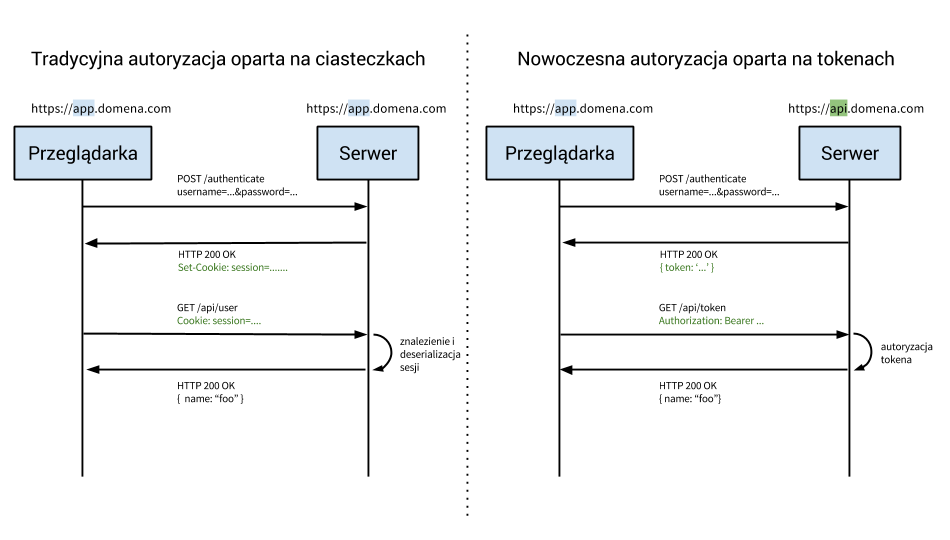
\includegraphics[scale=0.5]{tokenAuth.png}
  \caption{Diagram przepływu dla logowania tradycyjnego i tokenowego}
\end{figure}
\section{Technologie}
Aplikacja została podzielona na 2 części logiczne, którymi są:
\begin{itemize}
  \item Serwer
  \item Klient
\end{itemize}
Każda z nich używa innych technologii, ponieważ działają w różnych środowiskach np. klient pracuje jedynie w przeglądarce.
\subsection{Serwer}
Została napisana w języku C\# wykorzystując ASP.NET MVC 5 i ASP.NET Web Api 2. Statyczne pliki są udostępniane przy pomocy MVC, a reszta serwera została udostępniona w formie Web Service'u.\\ Silnik bazy danych, który został wykorzystany jest to Microsoft SQL Server 2012 w wersji Express LocalDB. Cała baza danych została zaprojektowana i wygenerowana przy pomocy Entity Framework 6, który także wspomaga wykonywanie zapytań do bazy danych. Zapytania w tej bibliotece nie wykonuje się bezpośrednio przy pomocy języka strukturalnego SQL, lecz pisząc kod i operując na encjach te zapytania są generowane w locie. Wielką zaletą tego typu rozwiązania jest możliwość przeniesienia aplikacji na inny silnik bazy danych bez zmiany jakiegokolwiek fragmentu kodu. Jedyną rzeczą, którą trzeba będzie wykonać to zmienić parametry połączenia. Jest to typowe rozwiązanie mapowania obiektowo-relacyjnego w skrócie ORM.
\subsection{Klient}
Klient został w większości przy pomocy biblioteki AngularJS. Jest to narzędzie napisane w JavaScript, które umożliwa tworzenie aplikacji za pomocą wzorca projektowego MVC, a także ułatwia tworzenie według koncepcji Single Page Application.\\ Interfejsu graficzny wykorzystuje bibliotekę Bootstrap, która nie tylko ładnie i schludnie wygląda, lecz przy zastosowaniu pewnych reguł zapewnia nam kompatybilność z innymi urządzeniami tj. telefony komórkowe, tablety, czytniki itd. Tego typu zgodność jest nazywana Responsive Web Desing i jest coraz częściej stosowana w internecie.\\ Wykresy są generowane przy pomocy HighCharts.js, który sprawia, że wykresy są proste w generowaniu.\\ Aplikacja została napisana modułowo i każdy takich modułów da się przetestować testami jednostkowymi, a wszystko dzięki narzuconemu schematowi przez AngularJS.
\section{Baza danych}
Jak wyżej zostało napisane baza danych to Microsoft SQL Server 2012 Express LocalDB
Poniżej projekt bazy danych.
\subsection{Diagramy przedstawiające zależności między tabelami}

\subsection{Opis tabel}
\paragraph[short]{ExpenseModels}
Przechowuje wydatki i przychody
\begin{itemize}
  \item Id int IDENTITY (Identyfikator)
  \item Comment nvarchar(max) (Komentarz)
  \item Cost decimal(18,2) (Wartość wydatku/przychodu)
  \item UserId nvarchar(max) (Identyfikator użytkownika)
  \item DateAdded datetime (Data dodania wydatku/przychodu)
  \item DateOfExpense datetime (Data wydatku/przychodu wprowadzona przez użytkownika)
  \item Title nvarchar(max) (Nazwa wydatku)
  \item DateModified datetime (Data modyfikacji wydatku/przychodu)
\end{itemize}
\paragraph[short]{LimitModels}
Przechowuje dane wyzwań
\begin{itemize}
  \item Id int IDENTITY (Identyfikator)
  \item Name nvarchar(max) (Nazwa wyzwania)
  \item Amount decimal(18,2) (Wartość wyzwania)
  \item From datetime (Data, od której zaczyna się wyzwanie)
  \item To datetime (Data, do której trwa wyzwanie)
  \item UserId nvarchar(max) (Identyfikator użytkownika)
\end{itemize}
\paragraph[short]{LimitModelTagModels}
Tabela łącząca tabele wyzwań z tagami
\begin{itemize}
  \item LimitModelId int (Id wyzwania)
  \item TagModelId int (Id tagu)
\end{itemize}
\paragraph[short]{SummaryModels}
Przechowuje dane podsumowań
\begin{itemize}
  \item Id int IDENTITY (Identyfikator)
  \item Name nvarchar(max) (Nazwa podsumowania)
  \item From datetime (Data, od której zaczyna się wyzwanie)
  \item To datetime (Data, do której trwa wyzwanie)
  \item Type int (Typ podsumowania)
  \item Scope int (Zasięg podsumowania np. roczne, miesięczne itd.)
  \item UserId nvarchar(max) (Identyfikator użytkownika)
\end{itemize}
\paragraph[short]{TagModelExpenseModels}
Tabela łącząca tabele wydatków/przychodów z tagami
\begin{itemize}
  \item ExpenseModelId int (Id wydatku/przychodu)
  \item TagModelId int (Id tagu)
\end{itemize}
\paragraph[short]{TagModels}
Tabela przechowująca tagi
\begin{itemize}
  \item Id int IDENTITY (Identyfikator)
  \item Name nvarchar(max) (Nazwa tagu)
  \item UserId nvarchar(max) (Identyfikator użytkownika)
  \item SummaryModelId int (Identyfikator podsumowania)
\end{itemize}
Pozostałe tabele są wykorzystywane przez standardowy mechanizm autentykacji ASP.NET MVC.

%%%%%%%%%%%%%%%%%%%%%%%%%%%%%%%%%%%%%%%%%%%%%%%%%%%%%%%%%%%%%%%%%%%%%%%%%%%%%%
%%%%%%%%%%%%%%%%%%%%%%%%%%%%%%% BIBLIOGRAFIA %%%%%%%%%%%%%%%%%%%%%%%%%%%%%%%%%
%%%%%%%%%%%%%%%%%%%%%%%%%%%%%%%%%%%%%%%%%%%%%%%%%%%%%%%%%%%%%%%%%%%%%%%%%%%%%%

%\bibliographystyle{plain}

%\bibliography{bibliography}

\end{document}
